
%remark 

\begin{theorem}[Tunnel Troll Theorem]
\label{TTT}
Let $\Xi$ be a deterministic unary oritatami system of delay $\delta = 1$. The following statements hold.
\begin{enumerate}
\item At arity $\alpha \geq 3$, if $S[i] = t$ (i.e. the tunnel that stabilizes $w[i]$ is not singular) and $S[i+1] \neq \blacksquare$, then $\#bc(C_{i-1}) > \#bc(C_i)$.
\item At arity $\alpha = 2$, if $m$ is the number of occurrences of $bt$ as a factor in $S[1..k]$ for an index $k$, then $\#bc(C_{0}) - m \geq \#bc(C_{k})$.
\end{enumerate}
\end{theorem}

In order to prove this theorem, we use the following three lemmas.
%Let us introduce some lemmas for proving Tunnel Troll Theorem.

%%%%%%%%%%%%%%%%%%%%%%%%%%%%%%%%%%%%%%%%%%%%%%%%%%%%

\begin{lemma}
\label{TTT_entrance_Tab}
Let $\Xi$ be a deterministic unary oritatami system at delay $\delta = 1$ and arity $\alpha =2$. 
Assume $\Xi$ stabilizes the transcript until $w[i-1]$. If $S[i+1] = b$ and $S[i+2] \in \{ t_s, t_o \} $, then $\#bc(C_{i-1}) > \#bc(C_{i})$.
\end{lemma}

\begin{proof}%[lemma \ref{TTT_entrance_Tab}]
See Fig.\ref{TTT_tunnel_direction}.
$S[i+2] \in \{ t_s, t_o \} $ means that $w[i+2]$ is stabilized by a tunnel section of type S or O.
Thus,  its predecessor $w[i+1]$ must be inside the tunnel section, that is, $n_1$ and $n_2$ must be occupied.
Free bonds of $w[i]$, if any, cannot be used in future by another bead $w[j]$ because otherwise the part of transcript $w[i..j]$ and the bond between $w[i]$ and $w[j]$ would form a closed curve and the curve would cross the path of $C_{i-1}$ between $n_1$ and $n_2$, contradiction.
%Binding capabilities that $w[i]$ supplies are inactive according to Jordan curve theorem on $n_1$, $n_2$, and $w[i]$.
Therefore, if $w[i]$ forms a bond at its stabilization $\#bc(C_{i-1}) > \#bc(C_{i})$ holds.
We now prove that $w[i]$ must form a bond.


Suppose $w[i]$ were stabilized without any bond, that is, by a tunnel.
For that the two points that are a neighbor of both $w[i-1]$ and $w[i]$ must be occupied already.
In addition, at least one of the neighbors of $w[i]$ must be free because $S[i+1] = b$.
Thus, only the case to be considered is Fig.~\ref{TTT_tunnel_direction} (middle) with $n_5$ being occupied (that is, $n_4$ is free).
In this case, before $w[i]$ is stabilized, at lest three neighbors of $n_2$ were free and hence, a bead at $n_2$ was provided with one free bond and could form a bond with $w[i]$. \qed

\end{proof}

\begin{figure}[tb]
  \begin{center}
    \begin{tabular}{ccc}
    
    
      \begin{minipage}{0.3\hsize}
      \centering
        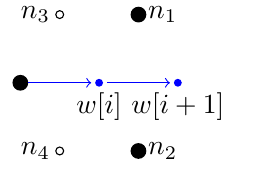
\begin{tikzpicture}
        \draw[->, white] (0:0)--(-120:1);
	 \draw[->,white] (120:0.8)--(120:0.1);%for adjustment
          
            \fill[blue] (0,0) circle [radius=0.05];
            \node[below] at (0,0) {$w[i]$};
            \node[below] at (0:1) {$w[i+1]$};

            \foreach \theta in {0}{
              \fill[transform canvas={shift=(\theta:1)},blue](0,0) circle [radius=0.05];
            }
            
            \foreach \theta in {60,-60,180}{
              \fill[transform canvas={shift=(\theta:1)}](0,0) circle [radius=0.1];
            }

            \foreach \theta in {120,-120}{
              \draw[transform canvas={shift=(\theta:1)}](0,0) circle [radius=0.05];
            }
            
            \draw[->, blue] (180:0.9)--(180:0.1);
            \draw[->, blue] (0:0.1)--(0:0.9);

            \node[transform canvas={shift=(60:1)},right] {$n_1$};
            \node[transform canvas={shift=(-60:1)},right] {$n_2$};
            \node[transform canvas={shift=(120:1)},left] {$n_3$};
            \node[transform canvas={shift=(-120:1)},left] {$n_4$};


         % \node at (0,-2) {$t_{0}$};
        \end{tikzpicture}
      \end{minipage}

      

      \begin{minipage}{0.3\hsize}
      \centering
        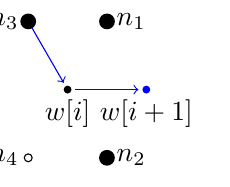
\begin{tikzpicture}
	\draw[->, white] (0:0)--(-120:1);
            \fill(0,0) circle [radius=0.05];
            \node[below] at (0,0) {$w[i]$};
            \node[below] at (0:1) {$w[i+1]$};

            \foreach \theta in {0}{
              \fill[transform canvas={shift=(\theta:1)},blue](0,0) circle [radius=0.05];
            }
            
            \foreach \theta in {60,-60,120}{
              \fill[transform canvas={shift=(\theta:1)}](0,0) circle [radius=0.1];
            }

            \foreach \theta in {180,-120}{
              \draw[transform canvas={shift=(\theta:1)}](0,0) circle [radius=0.05];
            }
            
            \draw[->, blue] (120:0.9)--(120:0.1);
            \draw[->, blue] (0:0.1)--(0:0.9);

            \node[transform canvas={shift=(60:1)},right] {$n_1$};
            \node[transform canvas={shift=(-60:1)},right] {$n_2$};
            \node[transform canvas={shift=(120:1)},left] {$n_3$};
            \node[transform canvas={shift=(-120:1)},left] {$n_4$};
            \node[transform canvas={shift=(180:1)},left] {$n_5$};

          %\node at (0,-2) {$t_{\pm 60}$};
        \end{tikzpicture}
      \end{minipage}

      \begin{minipage}{0.3\hsize}
      \centering
        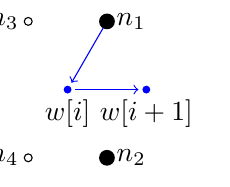
\begin{tikzpicture}
        \draw[->, white] (0:0)--(-120:1);
            \fill[blue](0,0) circle [radius=0.05];
            \node[below] at (0,0) {$w[i]$};
            \node[below] at (0:1) {$w[i+1]$};

            \foreach \theta in {0}{
              \fill[transform canvas={shift=(\theta:1)}, blue](0,0) circle [radius=0.05];
            }
            
            \foreach \theta in {60,-60}{
              \fill[transform canvas={shift=(\theta:1)}](0,0) circle [radius=0.1];
            }

            \foreach \theta in {180,-120,120}{
              \draw[transform canvas={shift=(\theta:1)}](0,0) circle [radius=0.05];
            }
            
            \draw[->, blue] (60:0.9)--(60:0.1);
            \draw[->, blue] (0:0.1)--(0:0.9);

            %\node[transform canvas={shift=(0:1)},below] {$n_0$};
            \node[transform canvas={shift=(60:1)},right] {$n_1$};
            \node[transform canvas={shift=(-60:1)},right] {$n_2$};
            \node[transform canvas={shift=(120:1)},left] {$n_3$};
            \node[transform canvas={shift=(-120:1)},left] {$n_4$};
            \node[transform canvas={shift=(180:1)},left] {$n_5$};

         % \node at (0,-2) {$t_{\pm 120}$};
        \end{tikzpicture}
      \end{minipage}
      
    \end{tabular}
    \caption{The three ways to enter a tunnel: (Left) straight, (Middle) obtuse, (Right) acute. The bead $w[i]$ is stabilized at the entrance and $w[i+1]$ is stabilized inside.}
    \label{TTT_tunnel_direction}
  \end{center}
\end{figure}


%%%%%%%%%%%%%%%%%%%%%%%%%%%%%%%%%%%%%%%%%%%%%%%%%%%%

\begin{lemma}
\label{TTT_exit}
Let $\Xi$ be a deterministic unary oritatami system of delay $\delta = 1$ and arity $\alpha =2$.
%Let $w[i]$ be a bead which is stabilized at the exit of a tunnel.
If $S[i+1..j+1] = bt^{(j-i-1)}b$ for some $i,j$ with $i \leq j-2$ and $S[j] \in \{ t_s, t_o\}$, then $\#bc(C_{j-2}) \geq \#bc(C_j)$, and hence, $\#bc(C_{i}) \geq \#bc(C_j)$.
If $i \leq j-3$, then the second inequality is strengthened as $\#bc(C_{i}) > \#bc(C_{j})$.
%if we assume $\#bc(C_{i-2}) - \#bc(C_{i-1}) = a$, then $\#bc(C_{i}) - \#bc(C_{i-1}) \leq a$.
\end{lemma}

\begin{proof}%[Lemma~ \ref{TTT_exit}]
Since the binding capability never increases inside a tunnel, we just need to consider the exit of a tunnel.
See Fig.\ref{TTT_tunnel_exit}. 
At least one of points $n_1$ or $n_2$ must be free because otherwise $w[j]$ would be inside of a tunnel, that is, $S[j+1]$ would not be $b$.



Let $m$ be the number of bonds $w[j-1]$ forms, that is, $\#bc(C_{j-2}) - \#bc(C_{j-1}) = m$.
We claim $\#bc(C_{j}) - \#bc(C_{j-1}) \leq m$.
Indeed, if both $n_1$ and $n_2$ are free (see Fig.~\ref{TTT_tunnel_exit}), the predecessor $w[j-1]$ must be bound to both beads at $n_3$ and at $n_4$ because both of them still have a free hand.
Hence, $m \geq 2$.
Since $\#bc(C_{j}) - \#bc(C_{j-1})$ is less than the arity, this difference is at most $m$.

If $n_1$ is occupied, then $n_2$ is free.
The predecessor $w[j-1]$ must be bound $n_4$.
Hence,  $m \geq 1$.
The bead $w[j]$ can increase the binding capability at most by 1 because one of its free neighbors would, $n_0$ or $n_2$, is to be occupied by the successor $w[j+1]$.
Therefore, $\#bc(C_{j}) - \#bc(C_{j-1}) \leq m$.
  


Thus,$\#bc(C_{j-2}) \geq \#bc(C_j)$ , and hence, $\#bc(C_{i}) \geq \#bc(C_j)$.
If $i \leq j-3$, then the second inequality is strengthened as $\#bc(C_{i}) > \#bc(C_{j})$ because $S[i+1] = b$, that is, $\#bc(C_{i}) > \#bc(C_{i+1})$ and $\#bc(C_{i+1}) \geq \#bc(C_j)$. \qed


\end{proof}

\begin{figure}[tb]
  \centering
    \begin{tabular}{cc}
    \centering
      \begin{minipage}{0.45\linewidth}
      \centering
        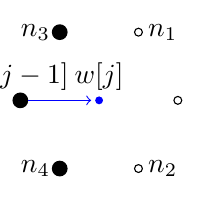
\begin{tikzpicture}
	\draw[white] (0:0) -- (120:1);
	\draw[white] (0:0) -- (-60:1);
	\draw[white] (0:0) -- (0:1);

            \fill[blue](0,0) circle [radius=0.05];
            \node[above] at (0,0) {$w[j]$};

            
            \foreach \theta in {120,-120,180}{
              \fill[transform canvas={shift=(\theta:1)}](0,0) circle [radius=0.1];
            }

            \foreach \theta in {0}{
              \draw[transform canvas={shift=(\theta:1)}](0,0) circle [radius=0.05];            }
            \draw (-60:1) circle [radius=0.05];
            \draw (60:1) circle [radius=0.05];

            \draw[->, blue] (180:0.9)--(180:0.1);



            \node[transform canvas={shift=(60:1)},right] {$n_1$};
            \node[transform canvas={shift=(-60:1)},right] {$n_2$};
            \node[transform canvas={shift=(120:1)},left] {$n_3$};
            \node[transform canvas={shift=(-120:1)},left] {$n_4$};
            \node[transform canvas={shift=(180:1)},above] {$w[j-1]$};

        \end{tikzpicture}
      \end{minipage}

      \begin{minipage}{0.45\linewidth}
      \centering
        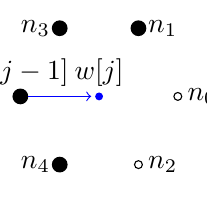
\begin{tikzpicture}

	\draw[white] (0:0) -- (120:1);
	\draw[white] (0:0) -- (-60:1);
	\draw[white] (0:0) -- (0:1);

            \fill[blue](0,0) circle [radius=0.05];
            \node[above] at (0,0) {$w[j]$};
            
            \foreach \theta in {120,-120,180,60}{
              \fill[transform canvas={shift=(\theta:1)}](0,0) circle [radius=0.1];
            }

            \foreach \theta in {0}{
              \draw[transform canvas={shift=(\theta:1)}](0,0) circle [radius=0.05];
            }
            \draw (-60:1) circle [radius=0.05];

            \draw[->, blue] (180:0.9)--(180:0.1);

            \node[transform canvas={shift=(0:1)},right] {$n_0$};
            \node[transform canvas={shift=(60:1)},right] {$n_1$};
            \node[transform canvas={shift=(-60:1)},right] {$n_2$};
            \node[transform canvas={shift=(120:1)},left] {$n_3$};
            \node[transform canvas={shift=(-120:1)},left] {$n_4$};
            \node[transform canvas={shift=(180:1)},above] {$w[j-1]$};

        \end{tikzpicture}
      \end{minipage}
    \end{tabular}
    \caption{Two kinds of exit of a tunnel: (Left) Both $n_1$ and $ n_2$ are free, (Right) One of $n_1$ and $n_2$ is occupied.}
    \label{TTT_tunnel_exit}
\end{figure}

%%%%%%%%%%%%%%%%%%%%%%%%%%%%%%%%%%%%%%%%%%%%%%%%%%%%


\begin{lemma}
\label{TTT_tunnelC_lemma}
Let $\Xi$ be a deterministic unary oritatami system of delay $\delta = 1$ and arity $\alpha = 2$.
If $S[i+2] = t_a$, the following statements hold.
\begin{enumerate}
\item If $w[i]$ forms at least one bond, $\#bc(C_{i-1}) > \#bc(C_{i+2})$.
\item If $w[i]$ does not consume any bond and $S[i] \in \{t_s, t_o \}$, $\#bc(C_{i-2}) > \#bc(C_{i+2})$.
\item If $w[i]$ does not consume any bond and $S[i] = t_a$, $\#bc(C_{i-3}) - 2 \geq \#bc(C_{i+2})$.
\end{enumerate}
%If there are indices $i,j$ such that $S[i..j+1]$ is either $bbt^{(j-i-1)}b$ and $S[i+2] = t_a$ or $bt^\ell bt^{j-i-1-\ell}b$ for some $\ell$ and $S[i+l+2] = t_a$, then $\#bc(C_{i-1}) > \#bc(C_j)$.
\end{lemma}

\begin{proof}

	We consider each statement. First we prove Statement 1.
	The bead $w[i+1]$ consumes one hand and provides nothing.
	If $w[i]$ forms two bonds, then even if $w[i+2]$ provides two free hands, $\#bc(C_{i-1}) > \#bc(C_{i+2})$.
	On the other hand, if it leaves a free hand, it will be used by $w[i+2]$, and hence, $w[i+2]$ does not increase the binding capability.
	Thus, $\#bc(C_{i-1}) > \#bc(C_{i+2})$.
	This argument actually work also for the case when $w[i]$ is stabilized rather by binding.
	
	Let us proceed to Statement 2.
	See Fig.~\ref{TTT_tunnelC_enter_usingBond}.
	Consider the case when $w[i]$ is stabilized by a tunnel section of type S or O.
	As prove in Lemma~\ref{TTT_exit}, $\#bc(C_{i-2}) \geq \#bc(C_{i})$.	The bead $w[i]$ leaves two free hand, it will be used by $w[i+2]$, and hence, $w[i+2]$ does not increase the binding capability.
	Thus, $\#bc(C_{i-2}) > \#bc(C_{i+2})$.
	This argument actually work also for the case when $w[i]$ is stabilized rather by binding.
	
	We finalize this proof by showing Statement 3.
	In order for $w[i]$ not to bind, $w[i-2]$ must have already used up its hands.
	The bead $w[i-1]$ consumes one hand and provides nothing.
	Thus,  $\#bc(C_{i-3}) - 1 \geq \#bc(C_{i})$.
	The bead $w[i+1]$ consumes one hand and provides nothing.
	Finally, $w[i+2]$ uses one hand of $w[i]$, and hence, does not increase the binding capability.
	Therefore, $\#bc(C_{i-3}) -2 \geq \#bc(C_{i+2})$.
	This argument actually works also for the case when $w[i]$ is stabilized rather by binding. \qed
\end{proof}

\begin{figure}[tb]
  \begin{center}
  \begin{tabular} {c c}
  \begin{minipage}{0.48\hsize}
  \centering
        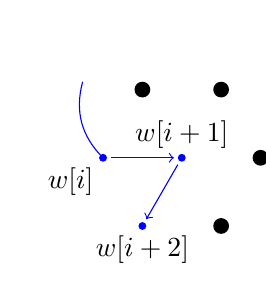
\begin{tikzpicture}
        \draw[->, white, shift=(180:1), shift=(120:1)] (120:0.9) -- (120:0.1);
          \foreach \theta in {60,-60,120,0}{
            \fill[transform canvas={shift=(\theta:1)}](0,0) circle [radius=0.1];
          }

          \fill[blue](180:1) circle [radius=0.05];
          \fill[blue](0:0) circle [radius=0.05];

          \draw[transform canvas={shift=(180:1)}, blue] (105:1) edge[bend right] (105:0);
          \draw[->, blue] (180:0.9) -- (180:0.1);
          \draw[->, blue] (-120:0.1) -- (-120:0.9);

          \node[below left] at (180:1) {$w[i]$};
          \node[above] at (0:0) {$w[i+1]$};
          \node[below] at (-120:1) {$w[i+2]$};
          \begin{scope}[shift=(-120:1)]
            \fill[blue](0,0) circle [radius=0.05];
            
          \end{scope}
        \end{tikzpicture}

	\end{minipage}
	
	\begin{minipage}{0.48\hsize}     
        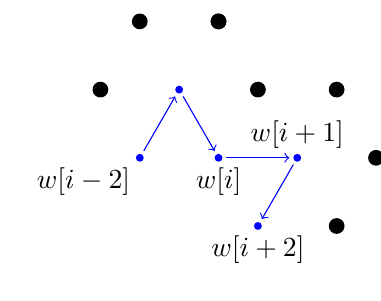
\begin{tikzpicture}
         \draw[->, white, shift=(180:1), shift=(120:1)] (120:0.9) -- (120:0.1);
          \foreach \theta in {60,-60,120,0}{
            \fill[transform canvas={shift=(\theta:1)}](0,0) circle [radius=0.1];
          }
          
          \foreach \theta in {60,60,120,180}{
            \fill[transform canvas={shift=(\theta:1)}, shift=(180:1)](120:1) circle [radius=0.1];
          }

          \fill[blue](180:1) circle [radius=0.05];
          \fill[blue](0:0) circle [radius=0.05];
          \fill[blue, shift=(180:1), shift=(120:1)](0:0) circle [radius=0.05];
          \fill[blue, shift=(180:1), shift=(120:1)](-120:1) circle [radius=0.05];

          
          \draw[->, blue] (180:0.9) -- (180:0.1);
          \draw[->, blue] (-120:0.1) -- (-120:0.9);
          \draw[->, blue, shift=(180:1), shift=(120:1)] (-60:0.1) -- (-60:0.9);
           \draw[->, blue, shift=(180:1), shift=(120:1)] (-120:0.9) -- (-120:0.1);

          \node[below] at (180:1) {$w[i]$};
          \node[above] at (0:0) {$w[i+1]$};
          \node[below] at (-120:1) {$w[i+2]$};
          \node[below left] at (-180:2) {$w[i-2]$};

          \begin{scope}[shift=(-120:1)]
            \fill[blue](0,0) circle [radius=0.05];
            
          \end{scope}
        \end{tikzpicture}
        \end{minipage}
        \end{tabular}
    \caption{The bead $w[i+2]$ is stabilized by a tunnel of type A. (Right) Moreover $S[i] = t_a$.}
    \label{TTT_tunnelC_enter_usingBond}
  \end{center}
\end{figure}


%%%%%%%%%%%%%%%%%%%%%%%%%%%%%%%%%%%%%%%%%%%%%%%%%%%%
%%
%%%%
%%%%%%
%%%%%%%%
%%%%%%%%%%%%%%%%%%%%%%%%%%%%%%%%%%%%%%%%%%%%%%%%%%%%

%Each bead in the transcript is bound either inside a tunnel or outside. If a bead is stabilized inside a tunnel, 
%then it has at most one free neighbor, and hence its successor it to be stabilized there.
%Moreover, if a bead is stabilized outside a tunnel, then its position is either an entrance of a tunnel or not.
%
%Tunnel sections have three possible shapes up to symmetry : straight($S$), obtuse($O$) and acute($A$) turn (Fig. \ref{fig:TTT_tunnel}), and we will consider each of those. 


%\begin{lemma}
%\label{TTT_neighbor_lemma}
%For unary transcripts at $\delta = 1$, if a bead has no free hand, then at least $\alpha + 2$ of its neighbors have to be occpied.
%\end{lemma}

Now we are ready to prove the Tunnel Troll Theorem.

\begin{proof}%{Proof of Tunnel Troll Theorem}
Let us first consider cases of $\delta \geq 3, \alpha = 1$. 
See Fig.~\ref{TTT_tunnel_exit}. Consider the stabilization of $w[i]$. 
This bead $w[i]$, once stabilized, shares two neighbors with its predecessor $w[i-1]$, which are denoted by $n_3, n_4$. 
Both of them have been already occupied because $S[i] = t$. 

Since $S[i+1] \neq \blacksquare$, at least one of the other three neighbors, denoted by $n_0, n_1, n_2$, must be free. 
Assume that in the neighborhood of $w[i]$, there are two beads with one free neighbor even after $w[i]$ is stabilized. 
Before the stabilization of $w[i]$, such a bead had two free neighbors, and hence, is provided with at least one free bond. 
Thus, $w[i]$ is to be bonded to these two beads, and it decreases the binding capability by at least 1. 
It now suffices to check that this assumption holds no matter how $n_0, n_1, n_2$ are occupied as long as at least one of them is left free. 

Next, we consider the case of $\delta = 2, \alpha = 1$. We assume there are indices $i$, $j$ such that $S[i+1..j+1] = bt^{(j-i-1)}b$.
If $S[i+2]$ is $ t_s$ or  $t_o$, then Lemma~\ref{TTT_entrance_Tab} implies $\#bc(C_{i-1}) > \#bc(C_{i})$ and  Lemma~\ref{TTT_exit} implies $\#bc(C_{i}) \geq \#bc(C_{j})$.
Thus, binding capability decreases by 1 per a factor $bt_s$ or $bt_o$.


%All $S[i+3..j]$ do not contain $t_a$; otherwise $S[i+4..j+1]$ contain $\blacksquare$.
%Therefore, $S[i+2] = t_a$.
Now, we assume $S[i+2] = t_a$.
Then, we have to make sure that one troll is not double-counted.
If $w[i]$ forms a bond, Lemmas~\ref{TTT_exit} and \ref{TTT_tunnelC_lemma} imply that binding capability decreases through this tunnel.

Assume $w[i]$ forms no bond.
If $S[i] \in \{t_s, t_o\}$, Lemmas~\ref{TTT_exit} and \ref{TTT_tunnelC_lemma} imply $\#bc(C_{i-2}) > \#bc(C_{i+2})$.
Observe that the bead $w[i-1]$ is at the entrance of the previous tunnel or inside.
It is when a bead is stabilized at the entrance of a tunnel that the troll of the tunnel decreases binding capability.
Thus, the inequality does not rely on the troll of previous tunnel.
If $S[i] = t_a$, Lemma~\ref{TTT_tunnelC_lemma} implies $\#bc(C_{i-3}) - 2 \geq \#bc(C_{i+2})$.
%The previous tunnel must be indeed a tunnel section of type A (see Fig.~\ref{TTT_tunnelC_enter_usingBond}).
This inequality involves two tunnels but its difference 2 enables us to consider that binding capability decreases by 1 through this tunnel. \qed
\end{proof}





%%%%%%%%%%%%%%%%%%%%%%%%%%%%%%%%%%%%%%%%%%%%%%%%%%%%%%%%%
%/////////////////////////////////////////////////
%%%%%%%%%%%%%%%%%%%%%%%%%%%%%%%%%%%%%%%%%%%%%%%%%%%%%%%%%


\subsection{Upper bounds on the length of conformation foldable deterministically at delay $\delta = 1$.}


\begin{theorem}[$\delta = 1, \alpha = 4$]
The terminal conformation of a deterministic unary oritatami system of $\delta = 1, \alpha = 4$ is of length at most $3n^2  + 3n + 1$.
\end{theorem}

\begin{proof}
Consider the moment when a bead, say $b$, is stabilized outside $\hexagon_O^n$ for the first time.
The bead must be bound a bead at the periphery of $\hexagon_O^n$ as depicted in Fig.~\ref{TTT_a4_first}.
%There is only one bead available to stabilize $b$ there, which is $b_1$. 
In order to avoid nondeterminism, the bead $b$ must not be attracted anyhow else by beads around. 

The point $p_1$ must be empty because a bead there would have at least two free neighbors and hence is provided with a free hand. 
If there is a bead at $p_2$, $n$ must be at least 2 so that the bead is not singular. 
Since $p_1$ is empty, this bead has at least one free hand, a contradiction. 
Thus, $p_2$ must be also empty. 
In the same way, we can easily show that the point $p_3$ must not be occupied by a non-singular bead. 
Suppose $p_3 = O$. 
The point $p_4$ must not be empty; otherwise the singular bead, at $O$, would have a free hand. 
However, then a bead at $p_4$ would be provided with a free hand, a contradiction. 
\qed
\end{proof}

\begin{figure}[tb]
 \centering
    \begin{tikzpicture}

	\fill (0,0) circle [radius=0.1];
        \fill[blue] (60:1) circle [radius=0.05];
        \fill (0:1) circle [radius=0.1];
        
	\draw[dotted, thick] (1, 0) -- ++(120:1);
      
      \draw[dashed] (180:2) -- (0:2);
      \draw[dashed, shift=(60:1)] (180:2.5) -- (0:1.5);
      \draw[->, blue] (60:0.1) -- (60:0.9);

	\node[above] at (180:1) {$p_1$};
	\node[left] at (-120:1) {$p_2$};
	\node[left, shift=(-120:1)] at (-60:1) {$p_3$};
	\node[right] at (-60:1) {$p_4$};

	\draw (180:1) circle [radius=0.05];
	\draw (-120:1) circle [radius=0.05];
	\draw (-60:1) circle [radius=0.05];
	\draw[shift=(-120:1)] (-60:1) circle [radius=0.05];

	\node at (0:2.5) {$n$};
	\node[shift=(60:1)] at (0:2) {$n+1$};
    \end{tikzpicture}
    \caption{The first bead out of $\hexagon_{O}^n$}
    \label{TTT_a4_first}
\end{figure}


%%%%%%%%%%%%%%%%%%%%%%%%%%%%%%%%%%%%%%%%%%%%%%%%%%%%%%%%%


\begin{theorem}[$\delta = 1, \alpha = 3$]
The terminal conformation of a deterministic unary oritatami system of $\delta = 1, \alpha = 3$ is of length at most $4n + 14$.
\end{theorem}



\begin{proof}
In this proof, we shall verify the claim that when the bead $w[i]$ is stabilized with $S[i] = b$ and $S[i+1] \neq \blacksquare$, if the circle of radius 2 centered at its predecessor $w[i-1]$ is free from the singular point, then $w[i]$ must form at least 2 bonds. 
Recall that the circle of radius 2 centered at the origin $O$, where the only candidate of singularity is, consists of 19 points including $O$. 
In order for the bead at $O$ to be singular, its $\alpha+1 = 4$ neighbors must be occupied. 
This means that there are at most 14 points where a bead find a singular bead within 2 points. 
Therefore, the claim, once proved, and the Tunnel Troll Theorem imply that all but at most 14 beads strictly decrease the binding capability. 
The binding capability of the seed is at most $3n$. 
Consequently, this theorem holds. 

Now let us verify the claim. 
Suppose $w[i]$ were stabilized by just one bond. 
There are three cases to be considered as depicted in Fig.~\ref{TTT_a3_w}, depending on the relative position of $w[i]$ to $w[i-2]$ and $w[i-1]$. 
Since $S[i] = b$, at least one of the four neighbors of $w[i-1]$ must be empty. 
If $n_3$ is free, then $w[i-2]$ must have used up all of its hands; otherwise, $w[i]$ would be stabilized also at $n_3$ nondeterministically, a contradiction. 
Thus, $\alpha + 2 = 5$ neighbors of $w[i-2]$, that is, all of its neighbors, must be occupied. 
Hence, $n_5$ is occupied. 
(All the remaining arguments are based on this ``merry-go-round'' occupation. This works only if the circle of radius 2 around $w[i-1]$ is free from the singular bead). 
In the same way, all the neighbors of $n_3$ turned out to be occupied in the clockwise order, but eventually, we would encounter a neighbor that is adjacent to also the point where $w[i]$ is supposed to go. 
Thus, $n_3$ must be occupied (in the left and middle cases). 
In the left case, $n_4$ is symmetric to $n_3$, and hence, it must be occupied, too. 
Since $S[i] = b$, $n_1$ or $n_2$ must be free; assume $n_1$ is. 
Going clockwise around $n_1$ implies that $n_{-1}$ is occupied, but the bead at $n_1$ has a free hand and would cause a nondeterminism. 

Let us focus on the remaining cases: middle and right. 
Suppose that among the 5 neighbors of $w[i]$ at which $w[i-1]$ is not, only one can be occupied. 
Otherwise, a bead without any hand is found at one of them, and staring from the point, merry-go-round occupies all the neighbors, but then $w[i+1]$ would lose its way to go. 
In the middle case, this means $n_0$ is free. 
Since $n_{-1}$ is free, so must be $n_2$. 
Repeating this, we get that both $n_4$ and $n_5$ are free, but then $w[i-2]$ would have a free hand and a free neighbor, attract $w[i]$, and cause a nondeterminism. 
Even in the right case, the points $n_1, n_0, n_2, n_4$ turn out to be free one after another likewise, but then $w[i-2]$ would have a free hand and neighbor, a contradiction. 
\qed

\end{proof}

\begin{figure} [tb]
  \begin{center}
  \begin{tabular}{c c c}
 \begin{minipage}{0.3\hsize}
 \centering
    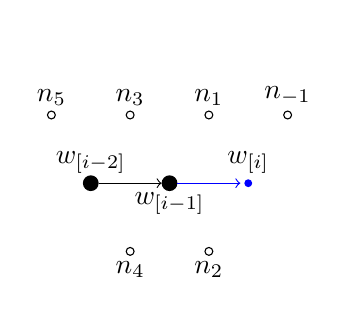
\begin{tikzpicture}
      \draw[white] (60:2) circle [radius=0.05];
      \node[right, white] at (60:2) {$n_{adj}$};
      
      \fill[shift=(180:1)] (0,0) circle [radius=0.1];
      \fill[shift=(180:0)] (0,0) circle [radius=0.1];
      
      \fill[blue](0:1) circle [radius=0.05];
      
      \draw[->] (180:0.9) -- (180:0.1);
      \draw[->, blue] (0:0.1) -- (0:0.9);

	\node[above] at (180:1) {$w_{[i-2]}$};
	\node[below] at (180:0) {$w_{[i-1]}$};
	\node[above] at (0:1) {$w_{[i]}$};

	\foreach \theta in {60,-60,120,-120}{
   	   \draw [shift=(\theta:1)] (0:0) circle [radius=0.05];
  	}
	 \draw [shift=(60:1), ] (0:1) circle [radius=0.05];
	  \draw [shift=(180:1),shift=(120:1)] (0:0) circle [radius=0.05];
 	\node[above] at (60:1) {$n_1$};
	\node[below] at (-60:1) {$n_2$};
	\node[above] at (120:1) {$n_3$};
	\node[below] at (-120:1) {$n_4$};
	\node[above, shift=(0:1)] at (60:1) {$n_{-1}$};
	\node[above, shift=(180:1)] at (120:1) {$n_5$};
    \end{tikzpicture}
    \end{minipage}
    
    \begin{minipage}{0.3\hsize}
    \centering
     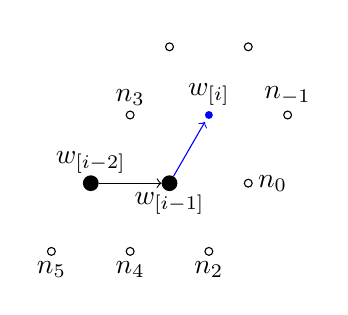
\begin{tikzpicture}
	\node[right, shift=(60:1), white] at (60:1) {$n_{adj}$};
      \fill[shift=(180:1)] (0,0) circle [radius=0.1];
      \fill[shift=(180:0)] (0,0) circle [radius=0.1];
      
      \fill[blue](60:1) circle [radius=0.05];
      
      \draw[->] (180:0.9) -- (180:0.1);
      \draw[->, blue] (60:0.1) -- (60:0.9);

	\node[above] at (180:1) {$w_{[i-2]}$};
	\node[below] at (180:0) {$w_{[i-1]}$};
	\node[above] at (60:1) {$w_{[i]}$};


	\foreach \theta in {0,-60,120,-120}{
   	   \draw [shift=(\theta:1)](0:0) circle [radius=0.05];
  	}
	\draw [shift=(60:1)] (0:1) circle [radius=0.05];
	\draw [shift=(60:1), shift=(60:1)] (0:0) circle [radius=0.05];
	\draw [shift=(60:1), shift=(120:1)] (0:0) circle [radius=0.05];
	  \draw [shift=(180:1),shift=(-120:1)] (0:0) circle [radius=0.05];
	
 	\node[right] at (0:1) {$n_0$};
	\node[below] at (-60:1) {$n_2$};
	\node[above] at (120:1) {$n_3$};
	\node[below] at (-120:1) {$n_4$};
	\node[above, shift=(60:1)] at (0:1) {$n_{-1}$};
	\node[below, shift=(180:1)] at (-120:1) {$n_5$};
    \end{tikzpicture}
    \end{minipage}
    
    \begin{minipage}{0.3\hsize}
        \centering
     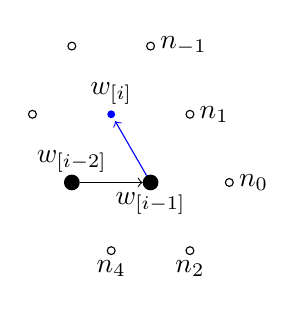
\begin{tikzpicture}
      
      \fill[shift=(180:1)] (0,0) circle [radius=0.1];
      \fill[shift=(180:0)] (0,0) circle [radius=0.1];
      
      \fill[blue](120:1) circle [radius=0.05];
      
      \draw[->] (180:0.9) -- (180:0.1);
      \draw[->, blue] (120:0.1) -- (120:0.9);

	\node[above] at (180:1) {$w_{[i-2]}$};
	\node[below] at (180:0) {$w_{[i-1]}$};
	\node[above] at (120:1) {$w_{[i]}$};


	\foreach \theta in {0,60,-60,-120}{
   	   \draw [shift=(\theta:1)] (0:0) circle [radius=0.05];
  	}
	\draw [shift=(120:1), shift=(60:1)] (0:0) circle [radius=0.05];
	\draw [shift=(120:1), shift=(120:1)] (0:0) circle [radius=0.05];
	\draw [shift=(120:1), shift=(180:1)] (0:0) circle [radius=0.05];
	
 	\node[right] at (0:1) {$n_0$};
	\node[right] at (60:1) {$n_1$};
	\node[below] at (-60:1) {$n_2$};
	\node[below] at (-120:1) {$n_4$};
	\node[right, shift=(120:1)] at (60:1) {$n_{-1}$};
    \end{tikzpicture}
    \end{minipage}
    \end{tabular}
    \caption{All possible directions of $w[i]$: straight, obtuse, acute.}
    \label{TTT_a3_w}
  \end{center}
\end{figure}




\begin{figure}[tb]
  \begin{center}
  \begin{tabular}{c c}
  \begin{minipage}{0.48\hsize}
  \centering
    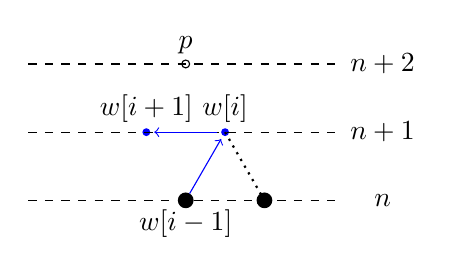
\begin{tikzpicture}
      	\fill (0,0) circle [radius=0.1];
        \fill[blue] (60:1) circle [radius=0.05];
         \fill[blue] (120:1) circle [radius=0.05];
        \fill (0:1) circle [radius=0.1];
      
      \draw[dashed] (180:2) -- (0:2);
      \draw[dashed, shift=(60:1)] (180:2.5) -- (0:1.5);
       \draw[dashed, shift=(60:2)] (180:3) -- (0:1);
      \draw[->, blue] (60:0.1) -- (60:0.9);
      \draw[->, blue, shift=(60:1)] (180:0.1) -- (180:0.9);
      
      \draw[dotted, thick, shift = (60:1)] (0:0) -- (-60:1);
      

	\node[above,shift=(120:1)]at (60:1) {$p$};

	\draw[shift=(120:1)] (60:1) circle [radius=0.05];

	\node at (0:2.5) {$n$};
	\node[shift=(60:1)] at (0:2) {$n+1$};
	\node[shift=(60:2)] at (0:1.5) {$n+2$};
	
	\node[below] at (0:0) {$w[i-1]$};
	\node[above] at (60:1) {$w[i]$};
	\node[above] at (120:1) {$w[i+1]$};
	\end{tikzpicture}
    \end{minipage}
    
    \begin{minipage}{0.48\hsize}
    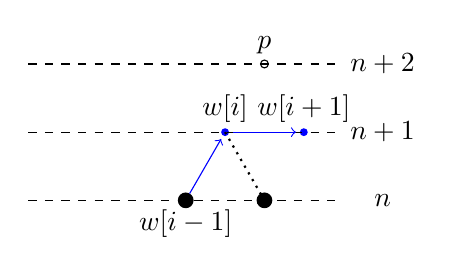
\begin{tikzpicture}
      	\fill (0,0) circle [radius=0.1];
        \fill[blue] (60:1) circle [radius=0.05];
         \fill[blue,shift=(0:1)] (60:1) circle [radius=0.05];
        \fill (0:1) circle [radius=0.1];
      
      \draw[dashed] (180:2) -- (0:2);
      \draw[dashed, shift=(60:1)] (180:2.5) -- (0:1.5);
       \draw[dashed, shift=(60:2)] (180:3) -- (0:1);
      \draw[->, blue] (60:0.1) -- (60:0.9);
      \draw[->, blue, shift=(60:1)] (0:0.1) -- (0:0.9);
       \draw[dotted, thick, shift = (60:1)] (0:0) -- (-60:1);
      

	\node[above] at (60:2) {$p$};

	\draw (60:2) circle [radius=0.05];

	\node at (0:2.5) {$n$};
	\node[shift=(60:1)] at (0:2) {$n+1$};
	\node[shift=(60:2)] at (0:1.5) {$n+2$};
	
	\node[below] at (0:0) {$w[i-1]$};
	\node[above] at (60:1) {$w[i]$};
	\node[above, shift=(0:1)] at (60:1) {$w[i+1]$};
	\end{tikzpicture}
    \end{minipage}
    \end{tabular}
    \caption{The moment when the transcript steps outside $\hexagon^n_O$.}
    \label{fig:ttt_d2}
  \end{center}
\end{figure}



\begin{theorem}[$\delta= 1, \alpha=2$]
A deterministic unary oritatami system of $\delta = 1, \alpha = 2$ can fold into an infinite conformation, but its transcript folds into the zig-zag conformation (Fig.~\ref{TTT_zigzag}) after its $(27n^2 + 9n +1)$-th bead.
\end{theorem}

\begin{proof}
 We assume $w[i]$ is the first bead stabilized outside $\hexagon^n_O$.
 See Fig.~\ref{fig:ttt_d2}.
 The next bead $w[i+1]$ is to be bound for stabilization.
 Hence, it goes to the west  or to the east (Fig.~\ref{fig:ttt_d2}).
 Once $w[i+2]$ is stabilized at $p$, the remaining transcript folds into the zig-zag conformation.
 In order to avoid this or nondeterminism, $w[i+2]$ must form two bonds; it thus decreases binding capability by 1.
 Until when a bead is stabilized outside $\hexagon^{n+1}_O$, binding capability never increases because of arity being 2 and of the Tunnel Troll Theorem.
 This means that, only at most $\#bc(C_0) \leq 2n$ times we can thus expand that hexagonal region.
 In other words, outside $\hexagon^{3n}_O$ the transcript cannot help but fold zig-zag. \qed
 
\end{proof}
